\header[h]{
    \headtitle{Chant des Pharmaciens} \label{chant-des-pharmaciens}
    %
    \insertComment{}{}
}

\enluminure{4}{\href{https://www.youtube.com/watch?v=chtyyX7MCk0}{C}}'est nous les pharmaciens qui venont vous trouver
\\Du fond des facultés pour vous administrer
\\Les capotes, les forceps, la poudre à faire bander
\\Et la vaseline Codex pour mieux faire pénétrer
\\La pine dans l'con comme un couteau dans l'beurre.
\\Les impuissants baiseront avec ardeur
\\Et si quelqu'un nous traite d'épicier
\\Son cul f'ra connaissance avec not'pied, avec not'pied.
\\\\\textbf{Refrain :}
\\Baisons ma mère
\\Devant, derrière
\\Les p'tites pucelles
\\Les vieilles maqu'relles
\\Les filles de rien
\\C'est nous les pharmaciens
\\\\Les littéraires sont des andouilles,
\\Les scientifiques sont des bizuths, oui des bizuths,
\\Vingt carabins n'valent pas les couilles
\\D'un pharmacien, ça c'est connu, ça c'est connu !
\\En avant, en marchant, en gueulant...
\\\\Et quand plus tard, dans nos boutiques,
\\Nous rappel'rons le bon vieux temps, le bon vieux temps,
\\Où nous bandions comme des triques
\\C'était l'époque des nos vingt ans, de nos vingt ans !
\\En avant, en marchant, en gueulant...
\\\\Les pharmaciennes ont la main douce
\\Elles épuiseraient un régiment, un régiment,
\\Il la leur faut bien de six pouces,
\\En largeur naturellement, naturellement !
\\En avant, en marchant, en gueulant...
\breakpage
Bien rembourrées devant, derrière,
\\C'est le propre de nos consoeurs, de nos consoeurs.
\\Un bon pilon, en la matière,
\\Ne remplace pas un bon baiseur, un bon baiseur !
\\En avant, en marchant, en gueulant...
\\\\Ainsi, baisons à tour de rôle
\\Ça ne sort pas de la maison, de la maison
\\Si quelqu'un attrape la vérole
\\Le 606 en aura raison, aura raison !
\\En avant, en marchant, en gueulant...
\\
% \begin{figure}[h!]
% \centering
%   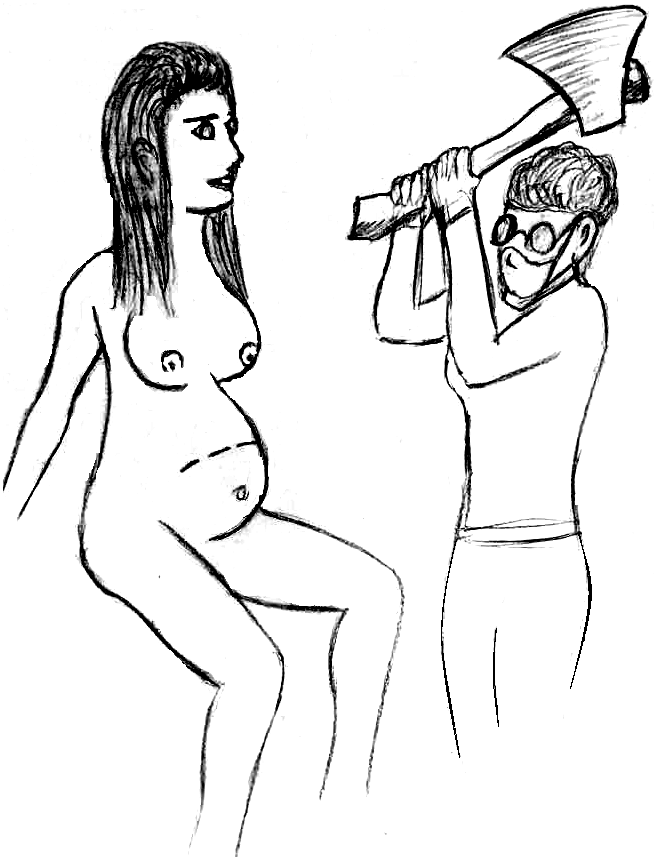
\includegraphics[width=0.8\textwidth]{images/cesarise_la.png}
%  \end{figure}
 
\breakpage